% file: DeepLearning_dump.tex
% Deep Learning, in unconventional ``grande'' format; fitting a widescreen format
% 
% github        : ernestyalumni
% linkedin      : ernestyalumni 
% wordpress.com : ernestyalumni
%
% This code is open-source, governed by the Creative Common license.  Use of this code is governed by the Caltech Honor Code: ``No member of the Caltech community shall take unfair advantage of any other member of the Caltech community.'' 
% 

\documentclass[10pt]{amsart}
\pdfoutput=1
%\usepackage{mathtools,amssymb,lipsum,caption}
\usepackage{mathtools,amssymb,caption}

\usepackage{graphicx}
\usepackage{hyperref}
\usepackage[utf8]{inputenc}
\usepackage{listings}
\usepackage[table]{xcolor}
\usepackage{pdfpages}
%\usepackage[version=3]{mhchem}
%\usepackage{mhchem}

\usepackage{tikz}
\usetikzlibrary{matrix,arrows,backgrounds} % background for framed option
\usetikzlibrary{arrows.meta}
\usetikzlibrary{cd}

\usepackage{multicol}

% ----------------------------------------------------------------------------------------
% 20180203

\usetikzlibrary{calc}

% ----------------------------------------------------------------------------------------


\hypersetup{colorlinks=true,citecolor=[rgb]{0,0.4,0}}

\oddsidemargin=15pt
\evensidemargin=5pt
\hoffset-45pt
\voffset-55pt
\topmargin=-4pt
\headsep=5pt
\textwidth=1120pt
\textheight=595pt
\paperwidth=1200pt
\paperheight=700pt
\footskip=40pt


\newtheorem{theorem}{Theorem}
\newtheorem{corollary}{Corollary}
\newtheorem{axiom}{Axiom}
%\newtheorem*{main}{Main Theorem}
\newtheorem{lemma}{Lemma}
\newtheorem{proposition}{Proposition}

\newtheorem{definition}{Definition}
\newtheorem{remark}{Remark}

\newenvironment{claim}[1]{\par\noindent\underline{Claim:}\space#1}{}
\newenvironment{claimproof}[1]{\par\noindent\underline{Proof:}\space#1}{\hfill $\blacksquare$}

%This defines a new command \questionhead which takes one argument and
%prints out Question #. with some space.
\newcommand{\questionhead}[1]
{\bigskip\bigskip
	\noindent{\small\bf Question #1.}
	\bigskip}

\newcommand{\problemhead}[1]
{
	\noindent{\small\bf Problem #1.}
}

\newcommand{\exercisehead}[1]
{ \smallskip
	\noindent{\small\bf Exercise #1.}
}

\newcommand{\solutionhead}[1]
{
	\noindent{\small\bf Solution #1.}
}

\title{The Deep Learning Dump}
\author{Ernest Yeung \href{mailto:ernestyalumni@gmail.com}{ernestyalumni@gmail.com}}
\date{19 July 2023}
\keywords{Deep Learning, Deep Neural Networks}
\begin{document}
	
\definecolor{darkgreen}{rgb}{0,0.4,0}
\lstset{language=Python,
	frame=bottomline,
	basicstyle=\scriptsize,
	identifierstyle=\color{blue},
	keywordstyle=\bfseries,
	commentstyle=\color{darkgreen},
	stringstyle=\color{red},
}
%\lstlistoflistings
	
\maketitle
	
If you find these notes useful, feel free to donate directly and easily through \href{https://www.paypal.com/cgi-bin/webscr?cmd=_donations&business=ernestsaveschristmas%2bpaypal%40gmail%2ecom&lc=US&item_name=ernestyalumni&currency_code=USD&bn=PP%2dDonationsBF%3abtn_donateCC_LG%2egif%3aNonHosted}{PayPal}. PayPal does charge a fee, so I also have a Venmo, \href{https://account.venmo.com/u/ernestyalumni}{ernestyalumni}, and CashApp (via email \url{mailto:ernestyalumni@gmail.com}).

Otherwise, under the \emph{open-source MIT license}, feel free to copy, edit, paste, make your own versions, share, use as you wish.    

\noindent gmail        : ernestyalumni \\
linkedin     : ernestyalumni \\
twitter      : ernestyalumni \\
		
\begin{multicols*}{2}
		
\setcounter{tocdepth}{1}
\tableofcontents
		
\begin{abstract}
Everything Deep Learning, Deep Neural Networks
\end{abstract}
		
\part{Deep Neural Networks}

\section{Cross Entropy Loss}

See \href{https://pytorch.org/docs/stable/generated/torch.nn.CrossEntropyLoss.html?highlight=crossentropyloss}{Pytorch "CrossEntropyLoss"}.

Consider the classification problem such that $y \in S$ where $S$ is some finite set, i.e. $S \in \textbf{FiniteSet}$. Let $C \equiv $ total number of "classes" or elements in this set $S$.

For what Pytorch calls \verb|minibatch| in the documentation for \href{https://pytorch.org/docs/stable/generated/torch.nn.CrossEntropyLoss.html?highlight=crossentropyloss}{"CrossEntropyLoss"}, let \verb|minibatch| $\equiv N$ for our notation (the reason is we can say we have $N$ samples in our batch).

$d_1, \dots, d_k$ with $K\geq 1$ for the $K$-dimensional case, with $K$ being the number of additional "features" for a single data point $x$. We've seen $K$ be denoted $D$ in other literature. 

The Pytorch literature says that the input into \verb|torch.nn.CrossEntropyLoss| is a "Tensor" of size (C) for unbatched input, (minibatch, C) or $(\text{minibatch}, C, d_1, d_2, \dots d_K)$. The documentation says the last "being useful for higher dimension inputs". I interpret this as being for a single data point with multiple features.

Consider these 2 examples: for a classification problem with $C = 3$ such as cat, dog, or mouse, if there are no additional features, we could imagine that for training data point $X$,

\[
X \mapsto h \in \mathbb{R}^C \mapsto y, \, y\in S \text{ s.t. } |S| = C
\]
where $h \in \mathbb{R}^C$ are the so-called "logits" generated by the "forward pass" (the linear transformations and nonlinear element wise mappings of the model) which then result into a prediction for a $y \in S$. The input is of size $(N, C)$ as there are no further additional features to consider.

Consider a grayscale image (i.e. each pixel has a single value for brightness, 0 to 255). Generalize this to each pixel having a value in $\lbrace 0, \dots P_b - 1 \rbrace$. If the image has "dimensions" $H \times W = 28 \times 28$ for example, then $d_1 = H$ and $d_2 = W$ and $K = 2$. So in this case the input dimensions are $(N, C, d_1 = H, d_2 = W)$.

\section{Gaussian Processes}
Yang (2021) for Tensor Programs I\cite{Yang2021}

\part{Recurrent Neural Networks}

\section{Long Short Term Memory, LSTM}

The \href{https://docs.nvidia.com/deeplearning/cudnn/api/index.html}{NVIDIA CUDNN Documentation}, in 7.1.2.8. \verb|cudnnRNNMode_t| says these following equations apply for the 4-gate Long Short-Term Memory (LSTM) network with no peephole connections, and for the default mode of \verb|CUDNN_RNN_DOUBLE_BIAS|:

\begin{equation}\label{Eq:NVIDIALSTM}
\begin{aligned}
& i_t = \sigma(W_i x_t + R_i h_{t-1} + b_{Wi} + b_{Ri}) = \sigma(W_i x_t + b_{Wi} + R_i h_{t-1} + b_{Ri}) \\
& f_t = \sigma(W_f x_t + R_f h_{t-1} + b_{Wf} + b_{Rf}) = \sigma(W_f x_t + b_{Wf} + R_f h_{t-1} + b_{Rf}) \\
& o_t = \sigma(W_o x_t + R_o h_{t-1} + b_{Wo} + b_{Ro}) = \sigma(W_o x_t + b_{Wo} + R_o h_{t-1} + b_{Ro}) \\
& c'_t = \tanh{ (W_c x_t + R_c h_{t-1} + b_{Wc} + b_{Rc})} = \tanh{ (W_c x_t + b_{Wc} + R_c h_{t-1} + b_{Rc})} \\
& c_t = f_c \circ c_{t-1} + i_t \circ c_t' \\
& h_t = o_t \circ \tanh{ (c_t)} 
\end{aligned}
\end{equation}
where $\circ$ denotes an element-wise operation.

Compare this with the expression given in \href{https://pytorch.org/docs/stable/generated/torch.nn.LSTM.html#torch.nn.LSTM}{PyTorch, LSTM} and they are similar, but $c'_t \equiv g_t$ and $\odot$ denotes the element-wise operation. In Eq. \ref{Eq:NVIDIALSTM}, \\
$x_t$ is input at time $t$, \\
$i_t$ is the so-called input gate, \\
$f_t$ is the so-called forget gate, \\
$g_t$ is the so-called cell gate, \\
$o_t$ is the so-called output gate, \\

and
\begin{equation}
\sigma \equiv \text{ sigmoid operator, s.t. } \sigma(x) = \frac{1}{ 1 + \exp{ (-1)} }
\end{equation}
is the sigmoid function.

Also, output hidden (state of each) layer $h_t$ can be multiplied by a learnable projection matrix $h_t = W_{hr} h_t$. 

Let us write Eq. \ref{Eq:NVIDIALSTM} in the following manner:

\begin{equation}
\begin{gathered}
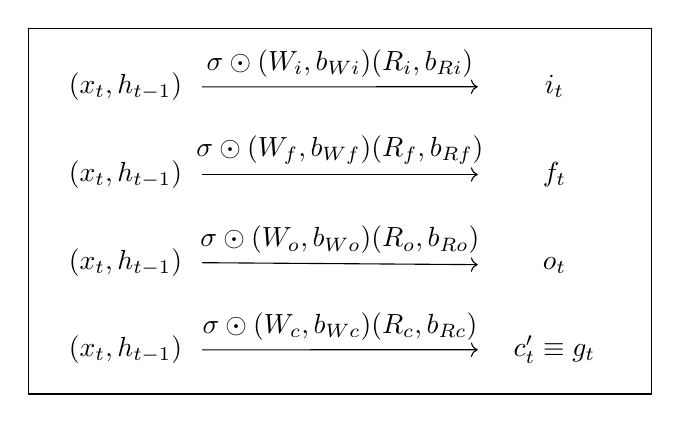
\begin{tikzpicture}[framed]
\matrix (m) [matrix of math nodes, row sep=1.5em, column sep=10em, minimum width=5.5em]
{
	(x_t, h_{t-1}) & i_t \\
	(x_t, h_{t-1}) & f_t \\
	(x_t, h_{t-1}) & o_t \\
	(x_t, h_{t-1}) & c'_t \equiv g_t \\
};
\path[->]
(m-1-1) edge node [above] {$\sigma \odot (W_i, b_{Wi})(R_i,b_{Ri})$} (m-1-2)
(m-2-1) edge node [above] {$\sigma \odot (W_f, b_{Wf})(R_f,b_{Rf})$} (m-2-2)
(m-3-1) edge node [above] {$\sigma \odot (W_o, b_{Wo})(R_o,b_{Ro})$} (m-3-2)
(m-4-1) edge node [above] {$\sigma \odot (W_c, b_{Wc})(R_c,b_{Rc})$} (m-4-2)
;
\end{tikzpicture} \\
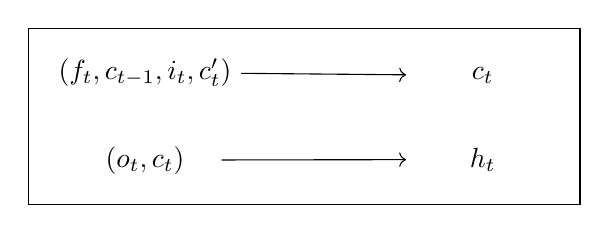
\begin{tikzpicture}[framed]
\matrix (m) [matrix of math nodes, row sep=1.5em, column sep=6em, minimum width=5.5em]
{
	(f_t, c_{t-1}, i_t, c'_{t}) & c_t \\
	(o_t, c_{t}) & h_t \\
};
\path[->]
(m-1-1) edge node [above] {$$} (m-1-2)
(m-2-1) edge node [above] {$$} (m-2-2)
;
\end{tikzpicture} \\
\end{gathered}
\end{equation}
From this we can clearly see that $\forall t \in \lbrace 0, 1, \dots T-1$ where $T$ is the \emph{sequence length} (Pytorch denotes this as $L =$ sequence length in the \href{https://pytorch.org/docs/stable/generated/torch.nn.LSTM.html#torch.nn.LSTM}{Pytorch LSTM documentation}) the inputs in are $(x_t, h_{t-1})$ and the output is $h_t$ and that $c_{t}$ is also effectively an output for the next time step $t+1$.

EY: 20230903 It is not clear however, what form does $c_{-1}$ takes that'd be necessary for the computation of $c_0$ for $t=0$. While one could maybe make some guess or ansatz about what $h_{-1}$ to use initially and compute $i_0, f_0, o_0$ to use for some initialized values for the operators $W$, $R$, and biases $b$'s, does one have to make a guess or ansatz about $c_{-1}$ as well?

\subsection{Interpreting NVIDIA \texttt{cudnn} Legacy API}

Let \\
$N = $ number of samples in a batch \\
$T = $ length of sequence \\
$D = $ number of features; size of a (single) input vector \\

Implied strides would be $(TD, D, 1)$. \\

$L=$ number of layers, $b= \begin{cases} 1 & \text{ if unidirectional } \\
	2 & \text{ if bidirectional } \end{cases}$ \\

$(bL, N, \begin{cases} P  & \text{ if LSTM of } \\ H & \text{ hidden size } \end{cases})$  \\

Consider strides: $( \lbrace NP, NH \rbrace, \lbrace P, H \rbrace, 1)$ \\

Cell dimensions or cells of rank $R$ \\
$(bL, N, H)$ \\

$x, hx, cx, W \mapsto \text{ forward } \mapsto y, hy, cy$ \\

$x,hx \mapsto \text{ backward on $W$ } \mapsto y, \partial W \equiv dW$ \\

if $o = [y, hy, cy] = F(x,hx, cx) = F(z)$, then \\

backwardData $\mapsto \left( \frac{ \partial o_i}{ \partial z_j } \right)^T \delta_{\text{out}}$, where $\delta_{\text{out}} \equiv \text{grad} l$ and $|\text{grad}l | = m\times 1$ \\

$\delta_{\text{out}} \equiv dy, dhy, dcy$ \\

gradient results $\left( \frac{ \partial o_i }{ \partial z_j} \right)^T \equiv dx, dhx, dcx$ \\

$y,dy, hx, dhy, cx, dcy, w \mapsto \text{ backward on Data } \mapsto dx, dhx, dcx$


\part{Transformer Networks}

Including \emph{Attention}

\section{Transformers}

\subsection{Input}

See Turner (2023) \cite{Turn2023}.

Let input data s.t. sequence of $N$ $\mathbf{x}^{(0)}_n$ of dim. $D$, $n = 0,1, \dots N-1$, $\mathbf{x}_n^{(0)} \in F^D$, where $F$ is some field (i.e. some data type such as float, double, etc.). \\

Let matrix $X^{(0)} \in F^{D\times N}$ or $\text{Mat}_F(D, N)$, a sequence of $N$ arrays of dim. $D$ collected into a matrix. \\

Let $M \in 0,1,\dots $ i.e. $M \in \mathbb{Z}^+$. \\

The goal is to map $X^{(0)}$ to $X^{(M)} \in \text{Mat}_F(D,N)$ i.e. $X^{(M)}$ of size $D\times M$ s.t. since $x_n = X_{;n}^{(M)}$ is a vector of features representing the sequence at location of $n$ in the sequence.

\subsection{Attention $A^{(m)}$ }

Consider output vector at location $n$, $\mathbf{y}_n^{(m)}$, where 
\begin{equation}
\mathbf{y}_n^{(m)} = \mathbf{x}^{(m -1)}_{n'} A^{(m)}_{n' n}, \quad \, n' = 0,1, \dots N-1
\end{equation} 
(Eq. (1) of Turner (2023) \cite{Turn2023}), where $A^{(m)}_{n' n} = A^{(m)}$ is called the attention matrix, $A^{(m)} \in \text{Mat}_F(N, N)$ and normalizes over its columns:
\begin{equation}
\sum_{n' = 1}^N A^{(m)}_{n' n}  =1
\end{equation}

\subsection{Projection of Q, K, V, queries, keys, and values}

Recall an input $\mathbf{x}_n = X^{(M)}_{;n} \in F^D$. Recall the linear transform resulting so-called queries or query vectors:
\[
\mathbf{q}^{(m)}_{h; n} = U^{(m)}_{q;h} \mathbf{x}^{(m-1)}_n \in F^K, \quad \, U^{(m)}_{q; h} \in \text{Mat}_F(K, D)
\]
where $h=0,1,\dots H-1$ with $H$ heads in Turner's notation (Turner (2023)\cite{Turn2023}). Compare this with NVIDIA's notation, \cite{NSAtn2023}, $i=0,1,\dots \texttt{nHeads} - 1$, so that $H \equiv \texttt{nHeads}$.\\

Generalize $K$ in dimensiosn $k\times D$ of $U^{(m)}_{q;h}$ to \texttt{qSize} $\equiv D_q$, i.e.
\[
\mathbf{q} \equiv \mathbf{q}^{(m)}_{h ; n} = U^{(m)}_{q;h} \mathbf{x}_n^{(m-1)} \in F^{D_q}, \quad \,  U^{(m)}_{q;h} \in \text{Mat}_F(D_q, D)
\] 

See \href{https://docs.nvidia.com/deeplearning/cudnn/api/index.html#cudnnSetAttnDescriptor}{7.2.45. \texttt{cudnnSetAttnDescriptor}}

\end{multicols*}

\begin{thebibliography}{9}

\bibitem{Yang2021} 
Greg Yang. "Tensor Programs I: Wide Feedforward or Recurrent Neural Networks of Any Architecture are Gaussian Processes." \href{https://arxiv.org/pdf/1910.12478.pdf}{arXiv:1910.12478v3} 8 May 2021

\bibitem{Turn2023}
Richard E. Turner. "An Introduction to Transformers". \href{https://arxiv.org/pdf/2304.10557.pdf}{arXiv:2304.10557v3 cs.LG 4 Jul 2023}

\bibitem{NSAtn2023}
NVIDIA. "7.2.45 \texttt{cudnnSetAttnDescriptor}". cuDNN API Documentation. \href{https://docs.nvidia.com/deeplearning/cudnn/api/index.html#cudnnSetAttnDescriptor}{7.2.45. \texttt{cudnnSetAttnDescriptor}}

\bibitem{SSB2014}
Hasim Sak, Andrew Senior, Francoise Beaufays. "Long Short-Term Memory Based Recurrent Neural Network Architectures For Large Vocabulary Speech Recognition." \url{https://arxiv.org/abs/1402.1128}

\end{thebibliography}
\end{document}
